\begin{frame}[fragile]{Funktion random\_poisson($\lambda$)}
  \begin{columns}
  \column{.59\textwidth}
    \begin{itemize}
  	\item Erzeugt poisson verteilte Zufallszahl
  	\item $\prod_{k}^{i=1}u_i \leq e^{-\lambda} < \prod_{k-1}^{i=1}u_i$
  	\item Sobald obige Bedingung zutrifft ist P($\lambda$) verteilte Zufallszahl k - 1
  \end{itemize}
  \begin{lstlisting}[language=python]
def random_poisson(lambd):
  k = 0
  u_list = []
  middle_value = exp(-lambd)
  while True:
    k += 1
    u_list.append(random.random())
    left_side = product(u_list)
    right_side = product(u_list[0:-1])
    if left_side <= middle_value < right_side:
      break
  return k - 1
\end{lstlisting}
\logopythonbottom
  \column{.39\textwidth}
    	\begin{figure}[h!]
    	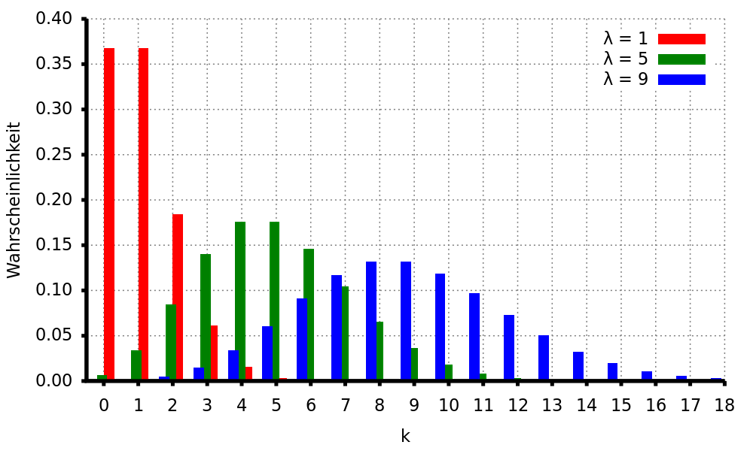
\includegraphics[scale=0.2]{lib_random_poisson_wahrscheinlichkeitsverteilung.png}
  			\caption{Wahrscheinlichkeitsverteilung der Poisson-Verteilung \tiny{(Wikipedia)}}
		\end{figure}
  \end{columns}
\end{frame}	